\subsection{Limitantes de performance}

De las etapas descriptas en la figura \ref{fig:lio-steps}, el m\'as costoso
en la implementaci\'on existente para GPU es el paso (j). En el c\'alculo de un sistema
de tama\~no medio, este paso solo representaba el 94\% del tiempo total. Esto hacia
que esta etapa llevara tanto tiempo como todos los dem\'as c\'alculos de SCF combinados, incluso
en las GPU m\'as veloces del mercado (Tesla K40, GeForce GTX 780). Adem\'as, en Fermi
el tiempo de c\'omputo de SCF era menor que en Kepler, yendo en contra de lo que prometen
las especificaciones de estos dispositivos.



A continuaci\'on detallaremos muchos de los cambios que fueron realizados para aumentar
la performance del c\'omputo de XC.

\subsection{Subsaturaci\'on de los SM}
La subsaturacion de los SM se da en los casos donde haya SM que est\'en listos para correr
c\'odigo pero que no puedan hacerlo porque tienen contenci\'on en algunos de sus recursos.
La m\'etrica usada para determinar esta saturaci\'on es la ocupancia de los SP.
Esta es la proporci\'on de threads activos sobre el total de threads disponibles de un bloque.

Existen en esta arquitectura principalmente tres recursos que, en un principio, parecen
ilimitados pero en realidad son finitos y compartidos por los procesadores de la GPGPU.
Estos son:
\begin{itemize}
\item Cantidad total de threads por bloque.
\item Cantidad total de registros usados por thread.
\item Cantidad de memoria compartida por bloque.
\end{itemize}

El mecanismo de scheduling de los SM funciona asignando un bloque a cada SM, que
va a correr sin preemption hasta que terminen todos sus threads asignados. Idealmente, cada
bloque cuenta con una cantidad de threads suficiente para poder esconder la latencia
de las ejecuciones mediante un cambio de contexto. La arquitectura GPGPU esta dise\~nada
para este fin, por lo cual se cuenta con un mecanismo de cambio de contexto de costo cero~\cite{NvidiaFermi} para
poder empezar a correr los threads de un warp diferente, del mismo bloque.
Si el bloque no cuenta con suficiente cantidad de threads para poner a correr de manera
concurrente, el SM va a forzosamente esperar que finalicen las operaciones de alta latencia
de estos warps sin nada que hacer mientras tanto. Si, por el contrario, se contasen con
miles de threads por bloque, entonces es posible que las operaciones que sirvan
para sincronizar los threads de todo un bloque en un punto espec\'ifico antes de proseguir
(un barrier) sean excesivamente costosas.

La arquitectura GPGPU de \nvidia organiza los registros de todos los threads en un \'unico
register file, com\'un a todos los bloques. Como cada thread usa decenas de registros para guardar
los c\'omputos intermedios, \nvidia decidi\'o unificarlos, ya que es muy variable la cantidad que va a usar
cada kernel de ejecuci\'on. Una de las grandes diferencias entre Fermi y Kepler es la cantidad m\'axima de
registros por thread. Mientras que Fermi permit\'ia hasta 63 registros, Kepler permite hasta 255. Esto
es positivo para poder correr bloques de pocos threads pero gran cantidad de registros. Por otro lado,
aumenta la presi\'on sobre el register file. Cuando se lanzan muchos threads
que puedan estar corriendo paralelamente entre todos los SM de la GPU, es posible que se supere
la cantidad m\'axima de registros presentes en el register file. Esto fuerza a que el scheduler
no pueda poner a ejecutar m\'as bloques que los que pueda soportar este recurso, dejando SP ociosos.

Finalmente, al igual que con los registros, la memoria compartida es un recurso limitado. Como
solamente se cuenta con hasta 48KB (Fermi-Kepler) de memoria de este tipo para ser repartida entre
todos los bloques que est\'en corriendo en todos los SM, el scheduler deber\'a decidir no poner a ejecutar
m\'as bloques simult\'aneamente que los que pueda soportar la cantidad de memoria compartida.

El problema de optimizar el c\'omputo del t\'ermino de intercambio-correlaci\'on tratado  cont\'o
con todos estos limitantes. Afortunadamente,
las herramientas de profiling usadas remarcan estos limitantes, haci\'endolas
fundamentales a la hora de evaluar como proseguir en la b\'usqueda de optimizaciones de c\'odigo.

\subsection{Cambios en el threading}
\label{threading}
%Cambiamos de blocks por puntos, a blocks por funci\'on.

De los 3 kernels que originalmente compon\'ian la iteraci\'on de XC en GPU, el que se encargaba
del c\'alculo de la densidad electr\'onica de la contribuci\'on de la energ\'ia de intercambio correlaci\'on
insum\'ia el 93\% del tiempo total de uso de la GPU. Minimizar el tiempo de ejecuci\'on de
esta funci\'on resultaba vital para poder disminuir el tiempo de iteraci\'on de SCF.

El cuello de botella fundamental en la ejecuci\'on radicaba en como se distribu\'ia el trabajo de computo
entre los kernels. La estrategia de paralelizaci\'on original determinaba la partici\'on
del grupo a resolver instanciando un bloque por cada punto ({$blockId.x < m$})
con una cantidad fija de threads (usando $threadId.x < BLOCK\_SIZE$)
Los threads serv\'ian para reutilizar la memoria compartida; cada thread le\'ia un
elemento de la matriz densidad ($C_{i,j})$) y luego lo compart\'ian con los
dem\'as threads.

\begin{figure}[htbp]
   \centering
   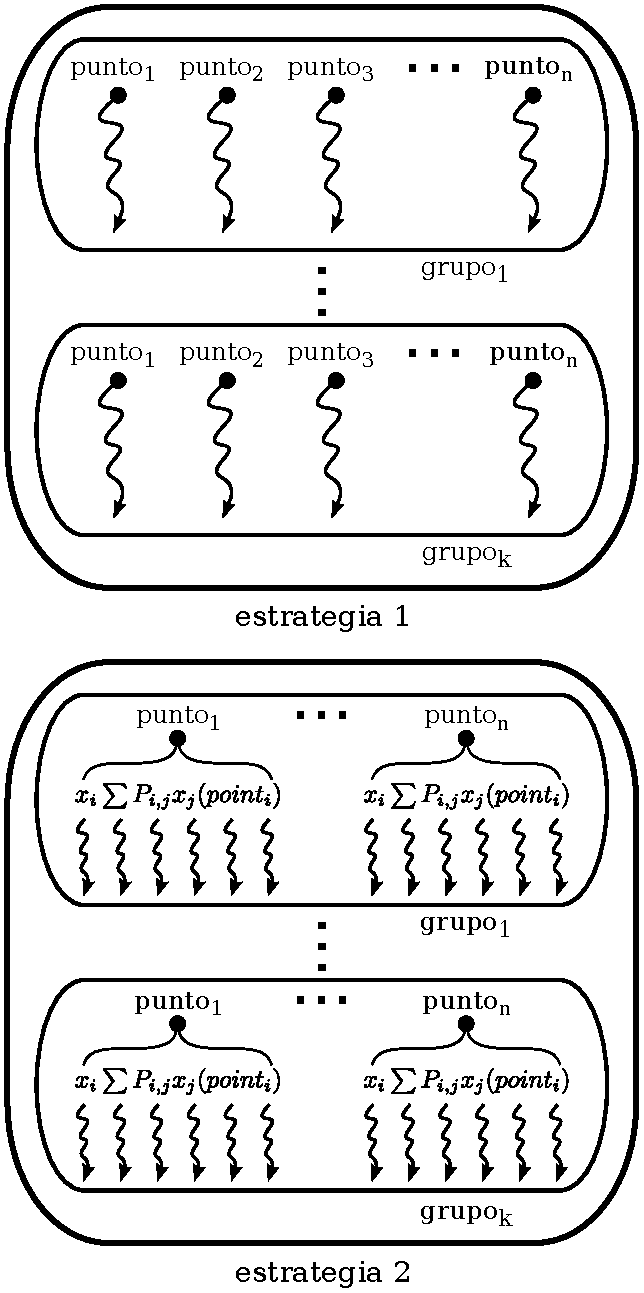
\includegraphics[width=250px]{images/cuda-parallelism.pdf}
   \caption{Estrategia original y modificada de paralelismo en el kernel de computo de la densidad
   electr\'onica computada durante $E_{XC}$.}
   \label{fig:cuda-xc-parallelism}
\end{figure}

El cambio m\'as importante para la performance provino de reconsiderar
la estrategia de paralelizaci\'on. La grilla con un bloque por punto con una cantidad
fija de threads tiene el problema de que, con bases con numerosas funciones, tiene que realizar
mucho trabajo por bloque. Esto causa que los SM est\'en ocupados constantemente
por kernels de larga duraci\'on. Lo que se busca es que los bloques realicen
menos trabajo por llamada, de modo que se puedan despachar a mas SM a medida
que estos terminen. En definitiva, lo que se busca es incrementar el throughput
de la placa. Esta estrategia se observa en la parte superior de la figura
\ref{fig:cuda-xc-parallelism}.

La nueva partici\'on del c\'alculo que se eligi\'o dispone un bloque por funci\'on,
de modo que cada thread $i$ realice la cuenta $F_i \sum_{j}^{i} F_j C_{i,j}$
y se compartan entre threads los valores de $F_i$ le\'idos.
Esta estrategia se ve en la parte inferior de la figura \ref{fig:cuda-xc-parallelism}.

La nueva estrategia permite una mucho mayor reutilizaci\'on de las lecturas a memoria
global, uno de los grandes limitantes de esta arquitectura.
La distribuci\'on original resultaba natural al problema, pero visto en detalle, esto
implicaba una cantidad elevada de lecturas a memoria global. Como cada thread realizaba un
punto dentro de un bloque, los $F_i$ que iba a leer no se pod\'ian compartir al ser
propios de cada punto. Como la cuenta ahora se realiza parcialmente por cada thread,
cada lectura de $F_i$ se agrega a la memoria compartida. El resto de los threads no van
a leer las funciones  de memoria global, sino de la compartida que ya cargaron los dem\'as. Esto
se traduce en que se realiza una lectura global y $BLOCK\_SIZE-1$ lecturas
de memoria compartida por cada thread. Como la latencia de acceso a memoria compartida
es, al menos, diez veces mas r\'apida que la memoria global~\cite{Demystifying}, esto incurre en grandes
beneficios con respecto a la velocidad del c\'omputo.

Este cambio solo es posible gracias al crecimiento de las memorias compartidas (16KB en la generaci\'on de
dispositivos existentes en implementaci\'on original, actualmente 48KB). Finalmente
esto tambi\'en se beneficia del incremento en tanto la cantidad de SM y la de SP por
SM. Todos estos factores permitieron una gran aceleraci\'on.

El otro cambio importantes fue partir en problema en m\'as bloques para las grupos que tengan
m\'as funciones significativas. Se decidi\'o agregar otra dimensi\'on a la grilla de bloques (\texttt{blockId.y}),
para determinar cuantos grupos de threads van a hacer falta para procesar completamente
todas las funciones de ese punto. Llamamos a este par\'ametro $altura\_bloques$. Se
calcula para cada partici\'on como $altura\_bloques = {m}/{BLOCK\_SIZE}$.
Para las particiones chicas, este valor no supera a 1. En los cubos y esferas m\'as
grandes (de los sistemas probados), la altura puede ser hasta 6. Esto significa una gran
cantidad de bloques adicionales con respecto al m\'etodo anterior.

\begin{figure}[htbp]
   \centering
   \includegraphics[width=\plotwidth]{plots/cuda/threading.png}
   \caption{Aceleraci\'on en veces de correr Hemoglobina en distintas arquitecturas con el cambio de estrategia.}
   \label{fig:threading}
\end{figure}

%%
%%

Despu\'es de haber hecho el cambio de la paralelizaci\'on, estudiamos realizar
m\'as de un punto por thread. Esto sirve para aprovechar un par de lecturas que son comunes
entre dos funciones. Con este cambio, se instancian menos bloques (la mitad de la dimensi\'on $y$
definida para esto) y se pueden ocultar algunas latencias de acceso, pero
cada grupo de threads lleva m\'as tiempo y usan m\'as registros. Esta estrategia es similar
a un loop unrolling manual, aplicado a la arquitectura GPU.

Un punto de intensa discusi\'on durante estos cambios es el valor de \textit{BLOCK\_SIZE}.
Para nuestro problema, decidimos utilizar un numero de threads por bloque m\'ultiplo del
tama\~no de un warp (32 threads). Esto permite estudiar como afectan en el tiempo de
procesamiento contar con uno o m\'as warps por bloque. Una ventaja de usar bloques de
32 threads, es que el costo de la sincronizaci\'on es exactamente cero. No se precisa
sincronizar nada puesto que los threads trabajan en lock-step sincronizados por warp.
Un bloque chico ademas nos permite usar mas memoria compartida por thread, dado que hay una
cantidad fija de memoria por bloque (entre 32KB y 64KB). Cuando se cuentan con muchos m\'as
threads, se debe reducir este uso por thread de modo que todos puedan ejecutar concurrentemente.

Dicho esto, la literatura~\cite{farberCuda} sugiere siempre que sea posible
usar bloques grandes y con threads lo m\'as independientes posibles. Una gran cantidad de threads
en un bloque permite tener muchos m\'as warps para schedulear de modo de esconder las latencias de
operaciones y de a accesos globales. Sin embargo, contar con muchos threads hace que las
sincronizaciones sean mucho m\'as costosas. Ademas, como cada SM no cuenta con preemption
de bloques, contar con muchos threads por bloque hace que los recursos se mantengan
por largos periodos.

Inicialmente, este tama\~no se hab\'ia fijado en 128 threads por bloque, 4 warps. Utilizando
mas memoria compartida en el esquema de paralelizaci\'on para disminuir accesos a memoria global,
este valor resulto demasiado elevado y disminu\'ia la posibilidad de ocupar todos los SM en dispositivos
Fermi y Kepler. Con solamente 32 threads, se pod\'ia maximizar la ocupaci\'on de los SM, pero hab\'ia
muchos m\'as bloques. Finalmente, luego de disminuir un poco el uso de memoria compartida por
bloque, usando algunas ideas descriptas a continuaci\'on, pudimos fijar este valor en 64 threads
por bloque. Se muestra en la figura \ref{fig:dbs-runtime} que tener solo un warp es bueno, pero
mejor a\'un es tener dos warps corriendo simultaneamente, porque
esto permite, con costo cero, poner a correr el otro para ocultar la latencia sin agrandar
demasiado el costo de la sincronizaci\'on.

Habiendo hechas todas las dem\'as optimizaciones detalladas en las secciones siguientes, evaluamos
\'unicamente este par\'ametro. Evaluamos un bloque de 32 threads hasta 128 threads por bloque,
el m\'aximo valor posible de modo que entre nuestro uso de memoria compartida.

\begin{figure}[htbp]
   \centering
   \includegraphics[width=\plotwidth]{plots/cuda/dbs.png}
   \caption{Tiempo de ejecuci\'on del c\'alculo de densidad corriendo Hemoglobina variando
   la arquitectura y tama\~no de \textit{BLOCK\_SIZE}.}
   \label{fig:dbs-runtime}
\end{figure}


\subsection{Reducci\'on anterior}
%Hubo que agregar reducci\'on de suma a nivel punto porque ya no se comparten mas la info
La reorganizaci\'on de la paralelizaci\'on del kernel del c\'alculo de la densidad creo la necesidad
de varios pasos de reducci\'on que antes se hac\'ian impl\'icitamente.

El primer paso, al ya no haber un bloque por punto, habr\'a que totalizar el c\'alculo de la
suma de todos los elementos de la columna que acabamos de procesar para obtenerlo. Para reducir,
vamos a reutilizar la memoria shared que empleamos en el c\'alculo de la energ\'ia anterior. Cada
thread va a poner el valor final del computo realizado en su posici\'on correspondiente en el
la memoria compartida. Esto luego se ejecuta como una reducci\'on en \'arbol, donde cada
thread suma el valor de la posici\'on $x$ con el valor en $2*x$, si fuera este valido. Esto
luego se repite por la mitad de los threads, hasta que solo el thread 0 lo ejecuta,
generando exactamente un valor por bloque, que lo va a terminar escribiendo en la memoria
global.

Esta t\'ecnica de reducci\'on es sumamente conocida para arquitecturas distribuidas, generando
la respuesta en $O(log_2(n))$ pasos. La literatura de CUDA~\cite{cudaReductions} sugiere t\'ecnicas adicionales para
minimizar a\'un mas el tiempo empleado en esta reducci\'on, pero considerando que hay, a lo sumo
6 operaciones, no hay necesidad de mejorar esto mas.

Como va a haber $altura\_bloque$ cantidad de escrituras para cada punto, va a entonces
hacer falta guardar estas cuentas parciales en memoria global. Para eso definimos una matriz
por cada uno de los par\'ametros que debemos acumular, con tama\~no id\'entico a la cantidad de bloques
del kernel del computo de densidad electr\'onica, para que cada uno de estos escriba \'unicamente en una posici\'on
un\'ivocamente identificada de este. Estas matrices luego son de tama\~no $O(\#_{puntos} * altura\_bloque)$,
menos de 1MB en el caso m\'as grande.

El siguiente paso de la reducci\'on consiste en acumular los $altura\_bloque$ valores descriptos
reci\'en en un solo por punto. Esto implica encontrar donde est\'an en las matrices temporales las
partes de las cuentas, agregarlas y calcular el potencial correcto. Esto genera finalmente los
coeficientes para calcular la actualizaci\'on de la matriz de Kohn-Sham y los factores para el
c\'alculo de la matriz de fuerzas.

Esto se refleja en el c\'odigo como una llamada a un nuevo kernel adicional, posterior a la
cuenta de la densidad y con m\'ultiples matrices temporales adicionales. Este kernel es sumamente
eficiente porque ya todo el trabajo pesado lo hizo el anterior. Solo se tiene que realizar
a lo sumo $altura\_bloque$ sumas y una llamada a la funci\'on que calcula el potencial y densidad,
un kernel corto de alta intensidad aritm\'etica que realiza solamente operaciones matem\'aticas.
Finalmente, la acumulaci\'on finaliza, generando un valor por cada punto, lo mismo que se produc\'ia
anteriormente pero utilizando mucho mejor los recursos del dispositivo.

Con respecto al costo de lanzar un kernel adicional, esto aprovecha que CUDA funciona de manera as\'incrona
con respecto al CPU, este kernel de reducci\'on se puede lanzar inmediatamente despu\'es de lanzar el
de c\'omputo de la densidad electr\'onica. Luego, como el c\'alculo de la densidad demora mas que
el overhead de lanzar el kernel de la reducci\'on, este tiene efectivamente un costo despreciable
ya que se pueden encolar en la GPU estas dos llamadas, que no dependen de nada que tenga que realizarse serialmente en CPU.
Desafortunadamente, como no se encuentra todo el c\'odigo de la resoluci\'on de un grupo en CUDA,
sino que tienen partes seriales en CPU intermedias, esta estrategia de aprovechar la asincronicidad
no se puede explotar para todos los kernels.

%%%%%%%%%%%%%%%

%\subsection{Tama\~no de los grupos}
%Un punto que afecta fuertemente el tiempo de ejecuci\'on del calculo de Intercambio Correlaci\'on
%es el tama\~no de los grupos que particionan los puntos del mallado. Los grupos son generados
%en base a constantes ajustables particulares a cada sistema, como se menciona en la seccion \ref{implementacion}.
%Estas constantes definen el tama\~no de cada cubo y el radio de cada esfera. El impacto de
%estos par\'ametros consiste en la cantidad de funciones significativas y puntos que van a ser
%capturados en cada grupo. Grupos muy chicos van a contar con pocas funciones y puntos, necesitando
%cientos o miles de grupos para poder representar un sistema de manera completa. Hacer grupos grandes,
%en cambio, permite que tengan miles de puntos y cientos de funciones, siendo aproximadamente un orden
%de magnitud m\'as grupos que en particiones chicas. Esto, sin embargo, no implica que todos
%los grupos sean grandes, simplemente que los cubos y las esferas cubrir\'an espacios mayores
%pero que dentro de estas puede haber pocos puntos.
%



\subsection{Cambios en los accesos globales}
\label{GuardarFunctionsGPU}
La arquitectura de las placas de v\'ideo est\'an pensadas entorno al poder de computo.
Las decisiones tomadas por los dise\~nadores de las GPGPU se concentran alrededor
de paralelismo a lo ancho, poniendo un gran \'enfasis en la cantidad de n\'ucleos. Luego,
se dispone de menor cantidad de espacio disponible en el \textit{die} para las memorias.

Esta decisi\'on implica que la amplia mayor\'ia de la memoria de la GPGPU se encuentra
localizada externa al procesador.  No solo esta f\'isicamente mas lejos, sino que
adem\'as la latencia para accederla es muy elevada. Es decir, el paradigma de
programaci\'on de las GPGPU gira entorno a esconder la gran latencia de los accesos
a las memorias globales.

As\'i como en CPU es importante realizar accesos alineados a memoria, en GPU es aun m\'as cr\'itico.
El termino coalescencia de memoria se define en GPU como la organizaci\'on de los accesos a memoria de secuencial, ordenada y predecible.
La l\'ogica detr\'as de esto es que cuando el GPU accede a memoria de manera alineada, puede traer
16, 32 o 64 elementos de 32 bits en una sola lectura\cite{cudaProgrammingGuide}, suficiente para
cada uno de los threads del warp. Si, en cambio, debe acceder de manera no
alineada a memoria o con threads que no acceden de manera predecible, entonces
se deber\'an serializar los accesos y separar en m\'ultiples transacciones a memoria global para satisfacer
el pedido. Este problema se agrava si se debe hacer accesos frecuentes
por cientos de threads, como es el caso de los bloques con gran nivel de paralelismo explicito.

En el paso del c\'alculo de la densidades el acceso a las funciones calculadas
se realizaba por columnas en vez de por filas. Esto ocasionaba que por cada acceso,
un warp tuviera que realizar 32 accesos secuenciales a memoria, ya que no se pod\'ian alinear
en una transacci\'on. Esto, ademas, se realizaba para las funciones, las derivadas y los
hessianos, por lo cual los accesos eran sumamente costosos. En el kernel original este comportamiento
no suced\'ia, ya que todos los threads realizaban cuentas para puntos independientes y no se compartian las
lecturas de las matrices. Esto aprovechaba las dimensiones originales de las matrices y hacian que las lecturas de
funciones fueran menos costosas, ya que se las usaba en el sentido correcto de la memoria (por filas).
Al haber cambiado la cuenta realizada para aprovechar mejor el threading (descripto en las secciones anteriores),
los accesos pasaron a ser por columnas y no por filas, rompiendo la coalescencia de las matrices. El
problema de los accesos se suele mitigar en CPU con el uso de las cach\'e, pero como las GPU cuentan
con L1 y L2 muy peque\~nas, el costo de acceder desalineado sigue siendo elevado.

Esto se soluciona transponiendo las matrices de valores de funciones, gradientes y hessianos.
La transposici\'on de matrices es un ejemplo sumamente estudiado por la literatura de CUDA
ya que ataca un punto d\'ebil de la arquitectura, el ancho de banda de transferencia. En la figura
\ref{fig:transpose} podemos ver que tanto en Fermi como en Kepler es muy notoria la diferencia
de performance, simplemente repensando los accesos a memoria. Kepler, al contar con una cach\'e L2
del doble de tama\~no que Fermi, lo mitiga un poco mas los accesos desalineados, pero todav\'ia recibe
grandes mejoras.

%Una cosa a tener en cuenta, pensando con respecto a la secci\'on anterior donde discutimos
%el cambio del threading, es que adem\'as se disminuyeron los accesos de lectura a las matrices de funcion.
%Al compartirlas entre threads usando las memorias shared, ahora se realizan muchos menos accesos a memoria global,
%ya que cada thread BLOCK\_SIZe elementos de cada matriz de funciones, pero todos salvo uno los leen de
%memoria compartida, ordenes de magnitud mas r\'apida que la global. Es decir, el impacto de este cambio
%es tan o m\'as importante a\'un que la coalescencia

\begin{figure}[htbp]
   \centering
   \includegraphics[width=\plotwidth]{plots/cuda/transpose.png}
   \caption{Aceleraci\'on en veces del kernel density de correr Hemoglobina en distintas arquitecturas habiendo transpuesto las matrices
   de funci\'on (incluyendo el costo de transponerlas).}
   \label{fig:transpose}
\end{figure}

Otra de las t\'ecnicas con la que cuenta CUDA para mitigar la latencia de acceso a memoria
es mediante el uso de memorias intermedias entre el procesador y la memoria global. Una de ellas es
la cach\'e de textura (siendo la otra la memoria constante). Esta es una cach\'e que
esta focalizada alrededor de los accesos a memoria de varias dimensiones.
Estas memorias reciben su nombre de su funci\'on principal, que es en el \'area de las
aplicaci\'ones de render de video. Los mapas de textura suelen ser grandes matrices que definen
tanto los colores sobre las superficies de los pol\'igonos como los relieves.
El detalle crucial de estas memorias es que un miss en estas cach\'e, provoca
que se traigan datos no solo contiguos en memoria, como pasa en las caches de
CPU normalmente, sino que ademas se traigan los datos en posiciones l\'ogicas contiguas,
es decir, variando las distintas dimensiones de la matriz subyacente.

Las memorias de textura se ajustan bien a los problemas de GPGPU, porque se relacionan
\'intimamente con los los mecanismos de paralelismo de CUDA. Como los problemas se pueden
dividir en bloques con threads en $x$, $y$, $z$, entonces tiene mucho sentido pensar
que las estructuras de datos subyacentes se van a acceder usando indices multidimensionales.

En nuestro problema, la memoria de textura se presenta como una soluci\'on para
los accesos bidimensionales de la matriz densidad para el grupo de puntos.
Como esta matriz debe ser multiplicada por todos los valores de las funciones,
derivadas primeras y segundas, se va a acceder a toda la matriz densidad mas de
una vez por cada thread. Adem\'as, como se va a usar toda la matriz, y esta suele
tener un tama\~no intermedio (es muy grande para memoria constante), el problema
suele entrar casi completamente en la memoria de textura.
La lectura bidimensional en este caso, se ajusta muy bien a los accesos por filas
y por columnas a la matriz.

\begin{figure}[htbp]
   \centering
   \includegraphics[width=\plotwidth]{plots/cuda/texture.png}
   \caption{Aceleracion del c\'alculo de densidad corriendo Hemoglobina en Fermi y Kepler
   usando memoria de textura para leer la matriz densidad.}
   \label{fig:texture}
\end{figure}

Como podemos ver en la figura~\ref{fig:texture}, esta optimizaci\'on aprovecha este
recurso \'unico de GPU. Sin embargo, esto agrega un factor mas que tenemos que tener en
cuenta a la hora de profilear el c\'odigo. Para administrar los accesos a
la memoria de textura, cada multiprocesador tiene m\'ultiples unidades de textura.
Cuando dependemos de sobremanera de la memoria de textura para esconder la latencia,
se presentan contenciones sobre el acceso a estas unidades. Esta cach\'e hay que usarla
solamente en los accesos mas costosos \'unicamente, ya que si intentamos pasar todos
los accesos a trav\'es de este, no solo no se ver\'ian mejoras, sino que seria un retroceso
completo de performance, como sucedi\'o cuando se intent\'o agregar adem\'as las matrices
de funciones a este m\'etodo.

%http://www.realworldtech.com/gt200/10/   << detalles sobre texture cache invalidation

%\subsection{Cambios en los pasajes de informaci\'on intrawarp}
%%Los shuffles que no anduvieron salvo en function
%La arquitectura SM35, junto con CUDA5, trajeron aparejadas una herramienta interesante
%para el manejo interno de los pasajes de informaci\'on intra-warp durante la ejecuci\'on.
%Las instrucciones de shuffle, como asi las denomina \nvidia, son instrucciones que facilitan
%el pasaje directo de un registro de un thread en un warp, a otro, en un solo ciclo de ejecuci\'on.
%Estas instrucciones existen en diversas maneras, con distintos propositos. Principalmente se
%utilizan para pasar de un thread al siguiente (modulo el warp size) un registro para poder seguir
%operando. Otro uso que puede tener mucho interes proximamente son las instrucciones de votaci\'on,
%donde se evalua un predicado para todos los threads, y se setea o limpia un bit en el resultado
%de respuesta si se cumplio el predicado para ese thread. Con esta herramienta, no es necesario
%acceder a memoria compartida para poder pasar minima informaci\'on dentro de cada warp.
%
%Nuestro uso de las funci\'ones de shuffle consistio en intentar eliminar lo m\'as que podiamos
%los accesos a la memoria compartida, una fuente de bloqueos porque, a pesar de que ya corre
%todos los bloques concurrentemente, leer elementos de ahi toman 4 ciclos en vez de uno solo
%como en las funci\'ones de shuffle.
%
%Probamos pasar de a un elemento y de a uno o dos vectores de 3 elementos, para comparar
%cuan notable era el impacto del acceso mas veloz.
%
%Finalmente concluimos que era una opcion valida para el pasaje de los valores de la funci\'on,
%pero que el overhead de uso para cosas como los hessianos de la funci\'on no justifica el uso.
%Adem\'as, como estas funci\'ones de shuffle solo estan presentes en las ultimas placas Kepler,
%consideramos que el aprovechamiento marginal de los recursos no era lo suficientemente meritorio
%de romper compatibilidad con las placas de la generacion Fermi anterior.


\subsection{Cambios en el almacenamiento de matrices temporales}
Una de las principales limitaciones de las GPGPU es la cantidad fija de memoria. Esta no se puede
expandir dado que esta soldada a la placa. Esto era aun m\'as notorio cuando las placas
contaban con menos de 1GB de memoria (A\~nos 2007-2008).
Para problemas de c\'alculo num\'erico, esto era un limitante muy serio; los problemas que
normalmente entraban en la memoria principal de un CPU, no entraban completos en las GPU.
La decisi\'on tomada por muchas aplicaciones de entonces es compensar esto calculando
datos intermedios y tir\'andolos al final; teniendo que ser recalculados en las pr\'oximas iteraciones.

Esta estrategia es claramente impr\'actica en CPU, puesto que se cuenta con mucha m\'as memoria
de uso general. En GPU era necesario por el faltante de memoria, pero puesto que estas cuentas se pueden
hacer m\'as r\'apido que en CPU, convirti\'endose entonces en una estrategia valida.

Cuando la aplicaci\'on original se concibi\'o, no hab\'ia siquiera placas GPGPU apuntadas a HPC, con
m\'as memoria disponible que los modelos de consumidores. Aprovechando estos recursos actuales,
desarrollamos un m\'etodos para poder almacenar las matrices de los valores de funciones y sus derivadas
en cada punto para cada grupo durante la ejecuci\'on de la aplicaci\'on, de modo de poder aprovechar
este recurso que originalmente era limitante pero ya no. Estas incluyen la matriz de funciones,
con una cantidad de elementos $O(puntos \times funciones)$, y si se usa el m\'etodo GGA
(\textit{Generalized Gradient Approximation}) para realizar los c\'alculos de DFT, tambi\'en se requieren
las matrices de gradientes y hessianos de las funciones ($O(3 \times puntos \times funciones)$ y
$O(6 \times puntos \times funciones)$ respectivamente).

Para poder determinar que cosas van a ser guardadas en memoria y que no, se determin\'o una heur\'istica
que define el orden de las particiones a solucionar. Esta heur\'istica estima que tama\~no van a
tener las matrices temporales a almacenar y ordena las particiones de menor a mayor. Esto
esta basado en el criterio de que, si bien es proporcional el tiempo de computo de estas matrices
temporales a la cantidad de funciones por grupo y cantidad de puntos (lo que determina el tama\~no
de la partici\'on), la constante es elevada. Determinamos entonces que es m\'as conveniente
aprovechar la memoria de la placa que almacena muchas matrices temporales de particiones chicas
a que almacene solamente un par de las grandes.

Para controlar la administraci\'on de memoria, se calcula si la placa dispone
con la suficiente memoria libre para guardar las matrices de funciones, y si puede, se almacenan de manera
permanente (hasta que la partici\'on se mueva a otro dispositivo o la liberaci\'on de recursos al
finalizar las iteraciones de SCF). Este mecanismo adem\'as es configurable de modo que una ejecuci\'on
pueda usar un porcentaje de la memoria con la que cuenta la placa, para poder correr m\'ultiples procesos de
simulaci\'on concurrentemente.

Un detalle a tener en cuenta es que, incluso si se maximiza el porcentaje de memoria usado para
cachear estas matrices, tal vez no alcanza para que quepa todo el sistema evaluado en memoria. Esto
se nota principalmente en la linea GeForce, que cuentan con aproximadamente entre un cuarto y la mitad
de la memoria global que tienen su equivalente en la linea Tesla. Esto es mitigado cuando se computa
m\'ultiples placas, que tambi\'en distribuyen el almacenamiento ademas del computo.


\begin{figure}[htbp]
   \centering
   \begin{subfigure}[b]{\plotwidthtres}
     \includegraphics[width=\plotwidthtres]{plots/cuda/global-detailed-fullereno.png}
     \caption{Entre 0 y 530 MB.}
   \end{subfigure}
   \begin{subfigure}[b]{\plotwidthtres}
     \includegraphics[width=\plotwidthtres]{plots/cuda/global-fullereno.png}
     \caption{Entre 0 y 4240 MB.}
   \end{subfigure}
   \caption{Aceleraci\'on del c\'alculo de una iteraci\'on de XC en funci\'on de la memoria de
   la placa usada para almacenar las funciones.}
   \label{fig:global-fullereno}
\end{figure}

Evaluamos el tiempo de ejecuci\'on de un sistema modelando un fullereno $C_{60}$, variando la
cantidad de memoria disponible para el cacheo. Los resultados se pueden ver en la figura \ref{fig:global-fullereno}.
Se puede observar que el almacenamiento de las matrices de funciones produce una mejora de casi el 25\% en el tiempo de ejecuci\'on
de toda una iteraci\'on de XC. Es interesante notar que son los primeros grupos los que causan mayor
diferencia en los tiempos de ejecuci\'on. Con 5.3 MB, se pueden guardar los 23 grupos mas peque\~nos del
fullereno $C_{60}$; de ah\'i en m\'as, el impacto de la mejora decae. Esto sucede porque en grupos
chicos el overhead del c\'alculo usando kernel de funciones es muy elevado en comparaci\'on a las
cuentas (se desperdician muchos threads). Este comportamiento se puede ver
bien en en la figura~\ref{fig:runtime-functions-fullereno}, donde se puede apreciar el importante
peso de los grupos chicos en el tiempo total del c\'alculo de las funciones. Decidimos no intentar
optimizar el c\'alculo ya que al almacenar las matrices este costo directamente se hace cero para
casi todos los grupos (dependiendo si el sistema entra entero o no en memoria).

\begin{figure}[htbp]
   \centering
   \includegraphics[width=\plotwidth]{plots/cuda/global-functions-acc.png}
   \caption{Fracci\'on del total del tiempo de c\'alculo de las matrices de funciones en una iteraci\'on en funci\'on
   del ordenada por el tama\~no acumulado de estas en un fullereno $C_{60}$.}
   \label{fig:runtime-functions-fullereno}
\end{figure}

Esta simple mejora permite explotar el hecho de que las placas hayan aumentado dram\'aticamente su
capacidad de almacenamiento, un recurso que hasta recientemente venia siendo un limitante podemos
convertirlo en una aceleraci\'on notoria.

\subsection{Cambios en las memorias compartidas}
%Cambiar los vec\_type4 por 3 en los accesos a la shared es mucho mejor, no hace falta alinear ahi
Otro de los problemas existentes del c\'odigo que quisimos atacar fue el mejor empleo de las
memorias shared. Estas son un recurso finito y muy importante, ya que son un limitante de
la ocupancia de los multiprocesadores. Como se pueden correr una cantidad de bloques que, a lo sumo,
no superen los 48KB de memoria shared simult\'aneamente entre todos, es imprescindible minimizar
el uso de la memoria shared de modo que no estemos subutilizando los SM.

Una cosa que probamos, con un grado de \'exito variable, fue disminuir el tama\~no de los vectores
donde almacenamos las derivadas direccionales. La manera de guardar las derivadas direccionales primeras
de las funciones que estaba implementada es usando tipos que agrupen en un solo elemento las tres derivadas
de cada punto, usando un cero al final para alinear en memoria, estrategia sugerida por la arquitectura CUDA para
maximizar la alineaci\'on y disminuir la cantidad de transacciones necesarias.
Es decir,$\nabla F_i = ( \frac{\partial F_i}{\partial x},\frac{\partial F_i}{\partial y}, \frac{\partial F_i}{\partial z}, 0 )$.
El m\'etodo GGA utiliza adem\'as las derivadas segundas de las funciones. Estas al ser funciones
Gaussianas de la base, son $C^\infty$, por lo que la matriz Hessiana es sim\'etrica. Entonces, va
a hacer falta \'unicamente guardar seis de las nueve derivadas segundas, las cuales se empaquetan de una manera
similar a la de las derivadas primeras, almacen\'andose en dos elementos con tres de estas derivadas
y un cero al final.

Un cambio que se intent\'o entonces fue llevarlos las derivadas de las funciones a que tengan tres elementos nada mas, para que ajustar
su uso real de memoria.  En las memorias globales, traer de a cuatro  valores consecutivos fuerza
al compilador a alinearlos a 16/32 bytes (simple y doble precisi\'on respectivamente). Esto presenta
grandes ventajas a la hora de hacer transferencias de memoria global en los accesos, por lo cual
decidimos dejarlo como estaban.

Sin embargo, este mismo criterio no aplica a las memorias shared de la GPGPU. Como los accesos
a estas memorias se realizan de a 4 bytes y no de a 16/32, entonces no tiene ninguna ventaja
en particular realizar el alineamiento; ya est\'an alineadas porque los elementos de cada punto
son flotantes de precisi\'on simple o doble (4 y 8 bytes respectivamente). Adicionalmente, como el
cuarto valor no tiene forma de marcarse como algo que no sea padding de alineaci\'on, todav\'ia se
opera normalmente con el usando operaciones vectoriales definidas para estos tipos, por lo que
eliminarlo ahorra una operaci\'on de c\'alculo. Mas a\'un, se presentan una disminuci\'on del 18\%
de la memoria compartida por thread (usando el esquema de compartir valores de funciones por punto
como fue descripto en la secci\'on \ref{threading}), sin ninguna desventaja por alineaci\'on a la hora de acceder a estos.
Principalmente esta mejora, en teor\'ia, permite
aumentar la cantidad de bloques corriendo concurrentemente en los SM, para poder eliminar
la limitaci\'on presente debido al uso concurrente de memoria compartida.

\begin{figure}[htbp]
   \centering
   \includegraphics[width=\plotwidth]{plots/cuda/shared-4vs3.png}
   \caption{Aceleraci\'on obtenida en Fermi y Kepler al reducir a 3 componentes los
   elementos en la memoria compartida.}
   \label{fig:shared4vs3}
\end{figure}

Como se puede observar en la figura~\ref{fig:shared4vs3}, se obtienen muy pocas ganancias al usar elementos
de 3 componentes con respecto a usar elementos de 4. Esto muestra que el limitante de concurrencia
de este kernel no pasa por falta de memoria compartida. Adem\'as, se puede apreciar que los
tiempos de acceso a los datos en estas memorias son realmente muy bajos, pudi\'endose ver
como con incluso un 18\% mas de operaciones de lecto-escritura, el tiempo de ejecuci\'on casi no varia. Por
otra parte, esto muestra tambi\'en que no hay diferencia en los tiempos de acceso a memoria compartida; buscar
tres o cuatro elementos es equivalente. Esto da la pauta de que se debe tener alineada en la global, pero
en la compartida se debe tener la menor cantidad de overhead posible, dadas las diferencias en los buses de acceso.


%\subsection{Cambios en los condicionales}
%La arquitectura CUDA representa un modelo de computo pensado en el procesamiento secuencial masivo
%de datos de punto flotante. Esto es herencia de su legado de placa gr\'aficas, que era un stream
%constante de datos. Al generalizar la arquitectura para que sea de prop\'osito general, entonces
%surge el problema de ejecuci\'on condicional. Como el resultado de la evaluaci\'on puede ser distinto
%para cada thread, entonces surge el problema de como ejecutar un warp en lockstep cuando algunos threads
%correr\'an la rama \texttt{true} y otros la rama \texttt{false}. La soluci\'on que adopta CUDA es la
%serializaci\'on impl\'icita. Los threads que no ejecutan el \texttt{true} correr\'an \texttt{NOP}
%y lo mismo se har\'a en el caso del \texttt{false}, al rev\'es.
%
%Esto trae aparejado una penalidad importante. Si esa bifurcaci\'on contiene mucho c\'odigo no trivial,
%entonces es evidente que se subutilizan importantemente los recursos disponibles.
%
%Habiendo varios de estos casos en los kernels presentes, decidimos utilizar una t\'ecnica sugerida
%por \nvidia. Esta consiste en hacer las operaciones normalmente, como si todos los threads cumplieran
%las condiciones del condicional y multiplicar por 1 o por 0 al resultado antes de acumular.
%Esto hace que las cuentas que no se ejecutaban antes ahora lo hagan pero que simplemente no aporten
%a la reducci\'on. Esta t\'ecnica elimina la existencia de la rama falsa de los condicionales, pero
%trae aparejada dos problemas no triviales.
%
%Uno de ellos es como solucionar el problema de los indices en los accesos a memoria.
%Un uso usual delas guardas condicionales es para evitar que el programa, si cumple ciertas condiciones,
%no acceda a memoria que esta mas all\'a de los limites definidos.
%Por ejemplo, si \texttt{threadId > arraySize}, entonces claramente
%no deber\'ia acceder a ninguna posici\'on mas all\'a de \texttt{array[threadId]},
%puesto que seria memoria invalida. Si eliminamos la guarda
%entonces los accesos a memoria pueden no quedar igual. Una soluci\'on consiste en multiplicar tambi\'en
%por 1 o por 0 la direcci\'on a la cual se va a acceder. Como CUDA maneja los arreglos de memoria
%como C (es decir, basados en 0 como primer direcci\'on), esta t\'ecnica es v\'alida para hacer
%siempre accesos correcto a memoria. El problema luego es en la coalescencia; como ahora algunos
%threads de un warp van a acceder a una posici\'on de memoria muy distinta a otros, entonces el procesado
%va a partir esos accesos en m\'ultiples transacciones. Esto puede hacer que la cuenta no solo no mejore
%la performance, sino que puede que la empeore sustancialmente. Se debe hacer un profiling caso
%por caso para poder estudiar el impacto en el kernel.
%
%El otro problema es en cuentas que pueden dar NaN (como el t\'ipico caso de divisi\'on por cero).
%Como, por est\'andar IEEE 754, los NaN hacen que todas las operaciones con ellos den NaN,
%entonces pueden propagarse por la cuenta, incluso en con multiplicaci\'on con cero del resultado.
%La soluci\'on m\'as evidente seria comprobar si son NaN antes de reducirlas, y si lo fueran, reemplazarlos
%por cero. Esto puede llegar a ser inevitable en muchos casos; en el nuestro, con replantear las cuentas,
%podemos evitarlos.

\subsection{Escalando m\'as all\'a de un GPU}
Una vez que fueron solucionados muchos limitantes de performance en los kernels del computo
de la densidad electr\'onica y del c\'alculo de la matriz de Kohn-Sham, nos encontramos en un punto donde
no fue posible determinar mejoras significativas en el c\'alculo para reducir tiempos.
Decidimos subir un nivel m\'as el paralelismo, de modo de poder solucionar m\'ultiples particiones
simult\'aneamente. Dado que es independiente el computo de cada partici\'on (salvo la acumulaci\'on
en la matriz de Kohn-Sham de salida y en la matriz de fuerzas interat\'omicas), nos pareci\'o que seria
interesante ver como escala distribuir el computo a lo largo de m\'ultiples GPU.

Para dividir el problema entre varios dispositivos usamos, al igual que en CPU, OpenMP. Definimos
una secci\'on paralela dentro del loop principal donde se soluciona cada grupo de modo que se
ejecutaran tantos threads como placas haya en la maquina. Cada
uno de los threads en el host se configurar\'a para una placa solamente. Esto se realiza con
una instrucci\'on del driver de CUDA (CudaSetDevice) que permite que durante toda la vida del
thread, todas las llamadas a kernels se realicen autom\'aticamente al mismo dispositivo.

CUDA permite que trabajar con m\'ultiples placas de esta manera sea bastante sencillo. Las variables
definidas como \texttt{\_\_device\_\_}, que residen plenamente en la GPU, son autom\'aticamente instanciadas
por cada dispositivo presente. De esta manera, es impl\'icito cual variable usa cada kernel; la que
esta definida para su dispositivo actual. Esto puede ser un problema si queremos lograr comunicaciones entre placas,
pero si las cuentas son independientes, es paralelismo de costo cero.

El principal problema que surge de uso de m\'ultiples dispositivos radica, al igual que en
CPU, en como distribuir la carga de los threads de modo tal que haya una cantidad de trabajo
similar, para minimizar los tiempos de idle. Este problema no es tan grave siempre y cuando
se utilicen placas id\'enticas dentro de la configuraci\'on del sistema ya que seria
el mismo tiempo si se corre en una o en otra. Un trabajo adicional de inter\'es ac\'a
radicar\'ia en el uso de t\'ecnicas de estimaci\'on de poder de computo para poder
distribuir el trabajo de manera equitativa entre modelos de placas heterog\'eneas, con distintas
configuraciones de memoria, cantidad de SM y anchos de banda.

Para distribuir las tareas utilizamos dos t\'ecnicas combinadas, una para distribuir las
tareas est\'aticamente y otra para redistribuirlas din\'amicamente de acuerdo al runtime de
cada tarea.


\subsubsection{Estimaci\'on de cargas est\'aticas}
Para la distribuci\'on est\'atica, usamos como estimador del runtime el tama\~no
de las matrices de funciones de un grupo. Esta heur\'istica resulta un acertado predictor
del tiempo de computo de todos los
kernels de un grupo confirmando que el problema actualmente es memory-bound. Esto se ve en la figura
\ref{fig:runtime-predictor}, como el tiempo de resoluci\'on de un kernel escala linealmente con
la cantidad de memoria necesaria para operar. Comparamos tambien contra el predictor usado
para estimar tiempo en CPU que se detallar\'a m\'as adelante en la secci\'on \ref{PredictorCPU}.

\begin{figure}[htbp]
   \centering
   \begin{subfigure}[b]{\plotwidthtres}
    \includegraphics[width=\textwidth]{plots/cuda/sizeingpu-predictor-hemo.png}
     \caption{Predictor de tiempo usando \textit{size\_in\_gpu}.}
   \end{subfigure}
   \begin{subfigure}[b]{\plotwidthtres}
    \includegraphics[width=\textwidth]{plots/cuda/cost-predictor-hemo.png}
     \caption{Predictor de tiempo usando funci\'on de costo.}
   \end{subfigure}
   \caption{Tiempos de ejecuci\'on de hemoglobina en Tesla K40 de acuerdo al costo del mismo seg\'un predictor.}
   \label{fig:runtime-predictor}
\end{figure}

Como podemos apreciar, esta directamente relacionado el tiempo de resoluci\'on con el tama\~no
de los elementos con los que trabaja. Esto da una pauta de la complejidad computacional del problema
que estamos resolviendo. Como al menos se necesita cada uno de los elementos de cada matriz de funciones
para resolver un punto de cada grupo. Al menos se deben hacer una lectura de cada matriz. Estas lecturas
son tan costosas que, incluso solo sabiendo el tama\~no de las matrices, podemos predecir aproximadamente
el tiempo de ejecuci\'on que va a tener un grupo.

El predictor usando el tama\~no, si bien es posible observar que tiene una buena correlaci\'on con el tiempo de ejecuci\'on,
no tiene la precisi\'on que tiene el predictor basado en la funci\'on de costo en CPU, visto en la figura~\ref{fig:comp-size-cost}.
No se pudo encontrar par\'ametros que permitan ajustarlo para que funcione en GPU. Como \nvidia no publica toda la informaci\'on
interna de los procesadores GPU y dada la cantidad de lugares adicionales donde se puede incurrir en latencias
imprevistas, al funcionar as\'incronos al CPU, no es posible predecir runtime con excesiva confianza dado \'unicamente
las cuentas a realizar. Al tener ambos predictores performance similares, se decidi\'o usar el m\'as sencillo, el
tama\~no de la matriz, como punto de partida para realizar una partici\'on del sistema en m\'ultiples GPU.

\subsubsection{Balance de cargas}
El balanceo de cargas \'optimo consiste en repartir $P$, el conjunto de problemas en
$n$ conjuntos disjuntos $P_i$, tal que $\bigcup_{i<n} P_i = P$. Este problema, conocido como PARTITION,
es NP-Hard en su versi\'on exacta, aunque son conocidos algoritmos pseudo-polinomiales para resolverlo.
La complejidad de ese algoritmo que usa programaci\'on din\'amica es $O(Nn)$, con $N$ el valor
de la suma de $P$ y $n$ la cantidad de elementos de $P$. Como nuestra m\'etrica de comparaci\'on para las
particiones es el runtime de estas expresados con precisi\'on de microsegundo, el costo computacional
de este algoritmo puede ser elevado en sistemas con cientos de particiones de miles de puntos.
La principal desventaja de usar \'unicamente este algoritmo es que no contempla, o no al menos
en sus versiones m\'as directas, el uso de recursos asim\'etricos. Es decir, resolver la partici\'on
optima del problema de particiones cuando se sabe que el costo de resolver $P_i$ en el dispositivo
$A$ es distinto a resolverlo en el dispositivo $B$. Por este motivo, no podemos particionarlo completamente
de manera est\'aticamente
usando este algoritmo y decidimos agregar usar una soluci\'on h\'ibrida est\'atica y din\'amica, reutilizando
la informaci\'on de runtime para decidir como rebalancear las particiones entre iteraciones de XC, luego
de haber hecho una aproximaci\'on inicial usando el predictor est\'atico antes mencionado.

Inicialmente definimos un orden para realizar toda la resoluci\'on del sistema y
se las distribuye de manera \textit{round-robin} entre todos los dispositivos, para generar la
partici\'on inicial y cargando a cada placa con una cantidad similar de tareas. Esto no significa
que todas tarden lo mismo, y es posible notarlo en las mediciones. Luego, utilizando el tama\~no
de los dispositivos como proxy del tiempo de ejecuci\'on, aplicamos una ronda del algoritmo de balanceo din\'amico
para terminar de balancear est\'aticamente. Esto lo podemos hacer ya que, como mostramos en la figura~\ref{fig:global-fullereno},
existe una fuerte correlaci\'on entre el tama\~no de las matrices de funci\'on y el tiempo de ejecuci\'on, la m\'etrica que realmente
nos interesa. El paso de balanceo din\'amico es necesario para solventar el problema de la distribuci\'on
round-robin con grupos grandes, donde el thread que tenga que resolver el grupo con mas puntos va a tardar
desproporcionadamente mas que los dem\'as. Un caso emblem\'atico es el cubo que contiene al \'atomo de hierro en la hemoglobina,
con mas de diez mil puntos y cientos de funciones de la base, con un tiempo de ejecuci\'on de al menos
dos ordenes de magnitud mas que el mas chico.

Para hacer el balanceo din\'amico, debemos determinar de ante mano la performance de cada
dispositivo con el que contemos. Para esto, se usa la tradicional t\'ecnica de definir un
caso de prueba representativo del problema, ejecutarlo en cada uno de los dispositivos y anotar
cuanto tarda en cada uno de ellos. Una gran ventaja de esto es que permite balancear f\'acilmente las
cargas cuando se realizan operaciones de doble precisi\'on en conjuntos de dispositivos que incluyan
placas Tesla y placas GeForce. En simple precisi\'on, los topes de linea de cada una pueden tener
performance similares (por ejemplo, GTX 580 y M2090, GTX 780 y K20), pero en doble precisi\'on
usualmente las Tesla suelen ser entre 2 y 6 veces mas veloces. Como las cuentas se realizan
o todas en precisi\'on simple, o todas en precisi\'on doble, es sumamente importante particionar el
sistema tomando todo esto en cuenta.

El problema ejemplar elegido en este caso es realizar $10$ iteraciones del kernel de c\'omputo de la matriz de Kohn-Sham.
Consideramos que realizar este c\'omputo nos da una evaluaci\'on
emp\'irica de los recursos necesarios para resolver este problema. Este kernel utiliza muchos
de los recursos del dispositivo: realiza gran cantidad de accesos a memoria a trav\'es
de la unidad de textura, usa principalmente instrucciones FMA, tiene una m\'axima ocupaci\'on de los SM
y tiene un uso total de la memoria shared. No contabilizamos las copias de memoria desde y hacia la
placa de los par\'ametros puesto que, al igual que en el c\'odigo de la simulaci\'on, casi la totalidad
de los datos se construyen directamente en la placa y se recuperan las matrices reducidas solamente al final
de la operaci\'on.

Teniendo las mediciones de tiempo para los $d$ dispositivos disponibles, se construye la matriz de
correcci\'on de tiempos de ejecuci\'on con los $d^2$ los coeficientes de correcci\'on para poder estimar el tiempo de
ejecuci\'on en el nuevo dispositivo. Si los dispositivos presentes son id\'enticos, como suele ser el caso
en clusters de computo cient\'ifico, entonces
la matriz va a tener solamente valores muy cercanos a 1, l\'ogicamente.

El pseudo c\'odigo del algoritmo de balanceo se detalla a continuaci\'on.
\begin{algorithm}
  \caption{Balanceo de duraci\'on de threads}
  \label{ThreadBalancing}
\begin{algorithmic}
  \State $tiempo_{\min} \gets tiempo[Thread_{\min}]$
  \State $tiempo_{\max} \gets tiempo[Thread_{\max}]$

  \While {$tiempo_{\max} /  tiempo_{\min} > k$}
    \State $\Delta T \gets (tiempo_{\max} - tiempo_{\min}) /2$
    \ForAll{$G_i \in Trabajos[T_{\max}]$}
    \State $T_{candidato} \gets  tiempo[G_i] * correccion[Thread_{\max}][Thread_{\min}] + costo\_migracion$
    \If{$|T_{candidato} - \Delta T| < T_{mejor\_candidato}$}
        \State $G_{mejor\_candidato} \gets G_i$
        \State $T_{mejor\_candidato} \gets T_{candidato}$
      \EndIf
    \EndFor
   \State Liberar la memoria de las matrices cacheadas de $G_{mejor\_candidato}$
   \State Mover $G_{mejor\_candidato}$ de $T_{\max}$ a $T_{\min}$
   \State Actualizar la duraci\'on total de $T_{\max}$ y $T_{\min}$, aplicando la correcci\'on de tiempos
  \EndWhile
\end{algorithmic}
\end{algorithm}

En el algoritmo \ref{ThreadBalancing} se definen dos constantes adicionales, $k$ y $costo\_migracion$.
$k$ representa el coeficiente de m\'axima diferencia de tiempo entre el thread de mas larga duraci\'on y el de menor
duraci\'on. Para nuestros usos, un valor de $k \approx 2\%$ es aceptable.
$costo\_migracion$ es un coeficiente que agrega un costo al migrar el grupo a otra placa, ya que va
a tener que recalcular las matrices de funciones que ya se guardaban en memoria. Cuando el trabajo cambie de placa, va a tener
que desalojarlas ya que, si bien es posible que entre las placas se accedan mutuamente a memoria global (utilizando
el direccionamiento unificado introducido en CUDA 5\cite{cudaProgrammingGuide})
no conviene dada toda la latencia introducida, que se adicionar\'a a lo largo de todas las iteraciones de la resoluci\'on.
Este coeficiente es equivalente a definir una penalidad por romper la \textit{afinidad} de las caches en CPU.

Otra ventaja de usar este algoritmo adicionalmente a la partici\'on est\'atica es que, si bien se considera la matriz
de correcci\'on, la finalidad es balancear la carga minimizando los tiempos, por lo que incluso si la estimaci\'on original
de performance relativa era err\'onea, igualmente se redistribuir\'an los distintos grupos.

%Adicionalmente, el algoritmo \ref{ThreadBalancing} agrega dos contadores para este balanceo. El contador de
%$ronda\_threads$ es el que sirve para balancear threads de a pares, necesario si hay mas de dos dispositivos.
%El contador de $ronda\_trabajos$ es el que balancea, para el thread m\'as r\'apido y el m\'as lento, los
%trabajos que van a migrar de un lado al otro. Es necesario agregar este contador por varios motivos. Por
%un lado, si se mueven demasiados trabajos de un momento a otro, tal vez la estimaci\'on final deje de ser realista,
%por lo que no tiene sentido seguir moviendo sin tener m\'as informaci\'on de otra corrida. Por otro lado, esta
%heur\'istica puede ciclar infinitamente si no se cumple la condici\'on de que se puedan balancear los tiempos
%con menos de diferencia $k$. En ninguno de nuestros casos de prueba nos hemos topado con que suceda esto, pero
%consideramos que es correcto dejarlo.

\begin{figure}[htbp]
   \centering
   \begin{subfigure}[b]{\plotwidthtres}
     \includegraphics[width=\textwidth]{plots/cuda/pre-group-split-differences.png}
     \caption{Previo al balance.}
     \label{fig:cuda-lio-imbalance-between-loads}
   \end{subfigure}
   \begin{subfigure}[b]{\plotwidthtres}
     \includegraphics[width=\textwidth]{plots/cuda/post-group-split-differences.png}
     \caption{Posterior al balance.}
     \label{fig:cuda-lio-imbalance-fixed}
   \end{subfigure}
   \caption{Comparaci\'on de los tiempos de ejecuci\'on para las distintas
   cargas asignadas a cada placa en el caso de Hemoglobina.}
   \label{fig:cuda-lio-imbalance}
\end{figure}

El rendimiento de esta optimizaci\'on se puede apreciar en la figura \ref{fig:cuda-lio-imbalance}. El predictor est\'atico
usado genera una partici\'on entre las cuatro placas con aproximadamente un 25\% de desbalance. En solamente
dos iteraci\'on del algoritmo \ref{ThreadBalancing}, se rebalancean las cargas entre placas moviendo tres trabajos, dos
de la placa 4 a la 2 y uno de la placa 3 a la 0. Con eso, las cargas quedan balanceadas a aproximadamente el 2\% de diferencia.
Este gr\'afico permite visualizar cual es la magnitud del error de estimaci\'on usando el predictor est\'atico definido anteriormente.

\subsubsection{Performance}
\label{cuda-multiplaca}

Resolver un sistema, en principio, debiera ser inherentemente paralelo; resolver para un grupo
no afecta resolver para otro. Sin embargo, escalar este problema entre m\'ultiples placas crea
nuevos problemas que no exist\'ian antes, como la concurrencia de escrituras sobre el bus de memoria.
Como cada dispositivo va a tener que copiarse un fragmento de la matriz global de densidad
y acumular en la matriz de Kohn-Sham de salida, va a existir una contenci\'on entre los threads que manejan
cada uno una GPU para leer y escribir en la memoria principal. Esto ocasiona que el speedup entre
m\'ultiples placas no sea lineal; al haber una cantidad limitada de trabajo que hacer en GPU y un fragmento de
resoluci\'on que necesariamente tiene que leer y escribir en memoria es una contenci\'on necesaria. Se puede
ver en la figura \ref{fig:4placas-simple} que no escala linealmente la aceleraci\'on del trabajo, los cuellos
de botella se notan a partir de la tercera placa, haciendo casi in\'util el uso de una cuarta.

\begin{figure}[htbp]
   \centering
   \includegraphics[width=\plotwidth]{plots/cuda/4placas-simple.png}
   \caption{Speedup en veces de correr Hemoglobina en 4 placas M2090 iguales en precisi\'on simple.}
   \label{fig:4placas-simple}
\end{figure}

Una importante excepci\'on a lo anterior es la realizaci\'on del c\'alculo en doble precisi\'on. La iteraci\'on
de XC se puede realizar tanto en simple como en doble precisi\'on, para minimizar los
errores de las operaciones. El costo de realizarlas en doble esta en la performance. Es notable
el tiempo adicional que compone cada iteraci\'on, por lo cual las simulaciones que lo usen van
a poder realizar como m\'aximo, aproximadamente un cuarto de la cantidad de iteraciones que la misma ejecutada en simple precisi\'on.
El c\'omputo utilizando precisi\'on doble tiene, sin embargo, ventajas en la escalabilidad entre placas.
Como los kernels en doble precisi\'on son \textit{compute-bound}, las copias de memoria son poco costosas
en relaci\'on a la resoluci\'on de los grupos (el tama\~no de las copias se duplica pero la potencia de c\'alculo se divide
por cuatro en Fermi y Kepler). Esto hace que haya poca contenci\'on en la memoria principal,
dado que hay menor concurrencia sobre estas. Podemos observar en la figura \ref{fig:4placas-doble} una clara mejora en los tiempos
de c\'alculo de los sistemas en doble precisi\'on entonces usando esta t\'ecnica de paralelismo, una mejora casi
lineal en la cantidad de dispositivos usados.

\begin{figure}[htbp]
   \centering
   \includegraphics[width=\plotwidth]{plots/cuda/4placas-doble.png}
   \caption{Speedup en veces de correr Hemoglobina en 4 placas M2090 iguales en precisi\'on doble.}
   \label{fig:4placas-doble}
\end{figure}

